%------------------------------------------------------------------------%
\chapter{Semiconductors basics}
%------------------------------------------------------------------------%
\section{Material distinction and energy gap}
{\bf Distinction betweeen materials}\\
In silicon-cristal electrons are subjected to periodical potential as a consequence to periodic disposition of atoms. We have bands of permitted energy level divided by gaps.\\
Importants bands are valence band VB ,that is the last band fully filled with electrons at 0 K, and conduction band CB ,that is the first band totally empty of electrons. Between this 2 bands there is the so called bandgap.\\
We can classificate all materials in 3 categories:\\
Metals           - $E_{gap}=0$ or "negative" and $\rho<10^{-2} \Omega$cm .\\ 
Semiconductors   - $E_{gap}=1eV$ and $10^{-2}<\rho<10^{5} \Omega$cm .\\
Isolators        - $E_{gap}>7eV$ and $\rho>10^{5} \Omega$cm.\\
\newline
%------------------------------------------------------------------------%
{\bf Energy gap function of T}\\
In Si $E_{gap}=1.12eV$ at room temperature (RT) but this value is a function of T; at high temperatures the silicon stretches and so does the periodical potential that influence the electrons.\\ 
The relation of $E_{gap}$ with temperature is
\begin{equation}
E_{gap}(T)=E_{gap}(0)-\frac{\alpha T^2}{\beta + T}
\end{equation}
where $\alpha$ and $\beta$ change from material to material.\\
We can consider a sensitivity parameter of the temperature as 
\begin{equation}
\frac{dE_{gap}(T)}{dT}=\frac{-2\alpha T(\beta+T)+\alpha T^2}{(\alpha + T)^2}
\end{equation}
At RT for Si we have a change of 25meV over 100 degrees.\\
\newline
%------------------------------------------------------------------------%
\section{Silicon concentration}
{\bf Conduction Band}\\
Using the effective band approximation we want to know the densitiy of states in CB or VB and after this the number of e or h in this bands.\\
Refering to the space of momentum we can say that
\begin{equation}
E-E_c=\frac{\hslash k_x^2}{2m_x}+\frac{\hslash k_y^2}{2m_y}+\frac{\hslash k_z^2}{2m_z}
\end{equation}
The iso-energetic surface in the space of momentum is an ellipsoid that is longer in the direction with effective mass higer. In the case 2 effective mass are equal we obtain a rotiation ellipsoide just as the case of Si in witch we have $m_x=m_z=0.19m_0=m_t$ and $m_y=0.92m_0=m_l$.\\
Observing that energy and the ellipsoide dimention are directly proportional we can say that all the points inside the ellipsoide have less energy than border ones.\\
The volume of the ellipsoide is 
\begin{equation}
\mathcal{V}=\frac{4}{3}\pi \sqrt{\frac{2m_x(E-E_c)}{\hslash^2}}\sqrt{\frac{2m_y(E-E_c)}{\hslash^2}}\sqrt{\frac{2m_z(E-E_c)}{\hslash^2}}=\frac{4}{3}\pi\frac{\sqrt{8m_xm_ym_z}}{\hslash^3}\sqrt{(E-E_c)^3}
\end{equation}
So the density of states will be 
\begin{equation}
N=\frac{\mathcal{V}}{(\frac{2\pi}{L})^3}\frac{1}{L^3}
\end{equation}
Making thefirst derivative of the equation by dE we can obtain finally 
\begin{equation}
g_c(E)=\frac{4\pi}{h^3}\sqrt{2m_xm_ym_z}\sqrt{E-E_c}\cdot 2 \cdot deg
\end{equation}
where the last 2 terms are a corrective coefficients for the spin and the degeneration of the material we consider.\\
We can say how many states are occupied only in a very specific case of thermodinamical equilibrium. If this condition is satisfacted we can use the Fermi-Dirac statistic 
\begin{equation}
f(E)=\frac{1}{1+e^{(E-E_f)/kT}}
\end{equation}
where $E_f$ is the Fermi level defined as the level at witch the prbability of occupation of an energy state by an electron is 1/2. $f(E)$ makes a smooth transition from 1 to 0 as the energy increases; the width of the transition is governed by kT.
That can be approximated with the Maxwell-Bolzmann statistic if $E-E_f>>kT$ 
\begin{equation}
f(E)\simeq e^{-\frac{E-E_f}{kT}}
\end{equation}
This is a good approximation if we are close to $E_c$ or at least well above $E_f$ at least a few kT.\\
Concentretion of electrons in CB is (under the condition of thermodinamic equilibrium)
\begin{equation}
n=\int^{+\infty}_{E_c} g_c(E)f(E)dE
\end{equation}
Making a change of variable as $x=(E-E_c)/kT$ and $\eta=(E_f-E_c)/kT$ we can write
\begin{equation}
n=\left[\frac{4\cdot 2\cdot deg \cdot \pi}{h^3}(kT)^{3/2}\frac{\sqrt{\pi}}{2}\right]\frac{2}{\sqrt{\pi}}\int^{+\infty}_0 \frac{\sqrt{x}}{1+e^{x-\eta}}dx=N_c\cdot F_{1/2}(\eta)
\end{equation}  
where $N_c$ is the density of states $F_{1/2}(\eta)$ is the Fermi-Dirac integral of order 1/2.\\
Assuming $x-\eta>>1$ (that is the M-B approximation) we arrive at 
\begin{equation}
n=N_c\frac{2}{\sqrt{\pi}}e^\eta \int^{+\infty}_0\sqrt{x}e^{-x}dx=N_ce^\eta=N_c e^{-\frac{E_c-E_f}{kT}}
\end{equation}
\newline
%------------------------------------------------------------------------%
{\bf Valence band}\\
Valence band of silicon has 3 sub-bands: heavy hole band and light hole that stay at VB level and the split-off band that stays 44meV under the VB. This 3 band mass are isotopic so the iso-energetic surface in the k space are spheres; bigger the sphere bigger the effective mass. We take into account for calculations only heavy hole band: 
\begin{equation}
E_v-E=\frac{\hslash^2 k^2}{2m_{hh}}\rightarrow\hat{k}_{hh}=\frac{\sqrt{2m_{hh}(E_v-E}}{\hslash}
\end{equation} 
as done before we calculate the volume of the sphere and the number of state per unit volume
\begin{equation}
\mathcal{V}=4/3\frac{\pi}{\hslash^3}\sqrt{8m_{hh}^3}\sqrt{(E_v-E)^3} 
\end{equation}
\begin{equation}
N=\frac{\mathcal{V}}{\frac{2\pi}{L}}\frac{1}{L^3}
\end{equation}
we can calculate the density of states as
\begin{equation}
g_V(E)=\frac{4\pi}{h^3}\sqrt{2m_{hh}}\sqrt{E_v-E}\cdot 2 \cdot deg
\end{equation}
we proceed as for the CB obtaining the total concentration per unit volume of holes that is 
\begin{equation}
p=p_{hh}+p_{lh}+p_{so}
\end{equation}
but the concentration of holes in the split-off band is negligible due to the distance from the valence band (the transition of 1-f(E) that stays in a few kT).\\
\begin{equation}
p\simeq N_v e^{-\frac{E_f-E_v}{kT}}
\end{equation}
\newline
%------------------------------------------------------------------------%
{\bf Intrinsic and estrinsic Silicon}\\
For intrinsic Si p=n and so we can calcuate $E_f$ from this eq as
\begin{equation}
E_f=\frac{E_c-E_v}{2}-\frac{kT}{2}\ln(N_c/N_v)=E_i 
\end{equation}
$E_i$ is the intrinsic level that stays in the middle of the gap (the correction is in the order of 0.3kT so negligible).\\
Putting 1.18 into p expression we obtain
\begin{equation}
p=n=\sqrt{N_cN_v}e^{-\frac{E_{gap}}{2kT}}=n_i
\end{equation}
$n_i$ is the intrinsic carrier concentration that has a strong dependance with T as it is involved in $N_c N_v$ and in $E_{gap}$.\\
From 1.11 by adding and subtracting $E_i$ and dividing the exponential in 2 parts we can write 
\begin{equation}
n=n_ie^{(E_f-E_i)/kT}\ \ \ \ p=n_ie^{(E_i-E_f)/kT}
\end{equation}
this are 2 expressions valid in general not only for intrinsic semiconductors.\\
We can introduce the law of mass action as 
\begin{equation}
pn=n_i^2
\end{equation}
For estrinsic semiconductors ,in the band diagram ,there is another band near to CB $(E_d)$ (or near to VB $(E_a)$ depending on the type of dope).\\
We want to extimate the position of $E_f$ in n-doped Si. We can write that $n=p+N_d^+$ where $N_d^+$ are the ionized donor concentration so
\begin{equation}
n=p+N_d(1-\frac{1}{1+1/2 e^{(E_d-E_f)/kT}})=p+\frac{N_d}{1+2e^{-(E_d-E_f)/kT}}
\end{equation}
the factor 1/2 it's a spin correction coefficient. At RT $E_d-E_f>>kT$ and p concentration is negligible in comparison with $N_d$ so $n\simeq N_d$ and from the law of mass action $p=n_i^2/N_d$. From this we can compute $E_f$ as 
\begin{equation}
E_c-E_f=kT\ln (N_c/N_d)
\end{equation}
Moving $E_f$ upwards some hypothesis falls: when $E_f$ reachs $E_d$ the complete ionization theory is not true anymore and from there further the M-B approximation is no longer valid.\\
\newline
%------------------------------------------------------------------------%
{\bf Fermi level dependence on temperature in doped semiconductors}\\ 

\begin{wrapfigure}{i}{0pt}
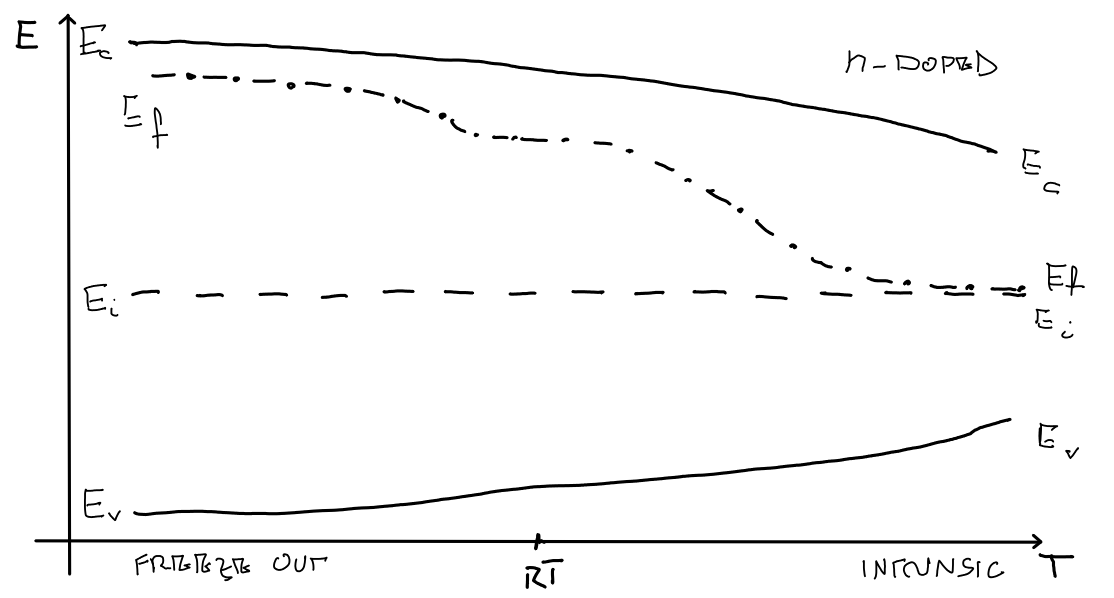
\includegraphics[width=0.5\textwidth]{E_f(T).png}
\end{wrapfigure}

With high T $E_g$ decreases and $E_f$ will move distant to $E_c$ following 1.18 until the hypothesis of negligible holes concentration decades and so at very high temperatures $E_f$ will tend asimptotically to $E_i$.\\
At very low temperature $E_f$ will increase until we reach the 0K where there is no conduction so $E_f$ has to stay a little bit higher than $E_d$.\\


%------------------------------------------------------------------------%
{\bf Low-temperature approssimation}\\

\begin{wrapfigure}{i}{0pt}
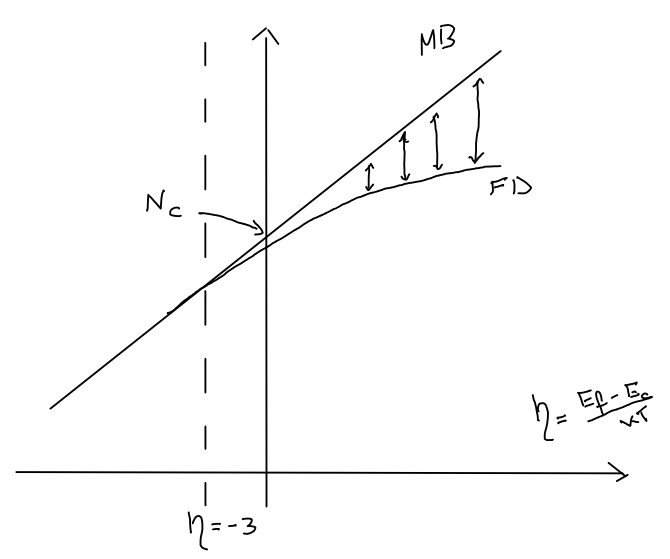
\includegraphics[width=0.35\textwidth]{mbfd.png}
\end{wrapfigure}

In the case of a material that has its Fermi level higher than the conduction band level we cannot use the M-B approximaton. The approximation we can do is a low-temperature one that trasforms the Fermi Dirac distribution into a step so
\begin{equation}
n=\int^{E_f}_{E_c}\frac{48\pi}{h^3}\sqrt{2m_t^2m_l}\sqrt{E-E_c}
\end{equation}
that multiplying and dividing the risult by $(kT)^{3/2}\sqrt{\pi}/2$ we obtain
\begin{equation}
n=N_c 2/3 \frac{2}{\sqrt{\pi}}\left(\frac{E_f-E_c}{kT}\right)^{3/2}=N_c 2/3 \frac{2}{\sqrt{\pi}}\eta^{3/2}
\end{equation}
In the graph below we can notice the difference between F-D and M-B distribution over $\eta$.\\
%------------------------------------------------------------------------%
\section{Current transport}
There are 2 most important mechanisms that generates current: drift and diffusion process.\\
Drift current is caused by the application of a electric field F; electrons are not only influenced by F but olso from scattering events so we can define a drift velocity (that is an average velocity) as 
\begin{equation}
v_d=\mu_n F
\end{equation}
So drift velocity is proportional to F with a constant $\mu_n$ called mobility that depends on doping concentration, temperature and dimensionality of the system taking in account all scattering events.It's important to note that in a bulk of doped Si if we are near the surface the mobility is much lower than the inside (dimensionality).\\
Mobility has a drop for Si around doping concentration of $\simeq 10^6 cm^{-3}$ beacuse at that level scattering with impurities becomes dominant in respect of thermal scattering.\\
Increasing too much F we arrive at the phenomena of velocity saturation ($\simeq 10^7 cm/s$) caused by scattering with high energetic optical phonons.\\
The density current caused by drift process is 
\begin{equation}
J=(qn\mu_n + qp\mu_p)F=\sigma F=F/\rho
\end{equation}
where $\sigma$ is the conductivity of the material and $rho$ is the resistivity.\\

\begin{wrapfigure}{i}{0pt}
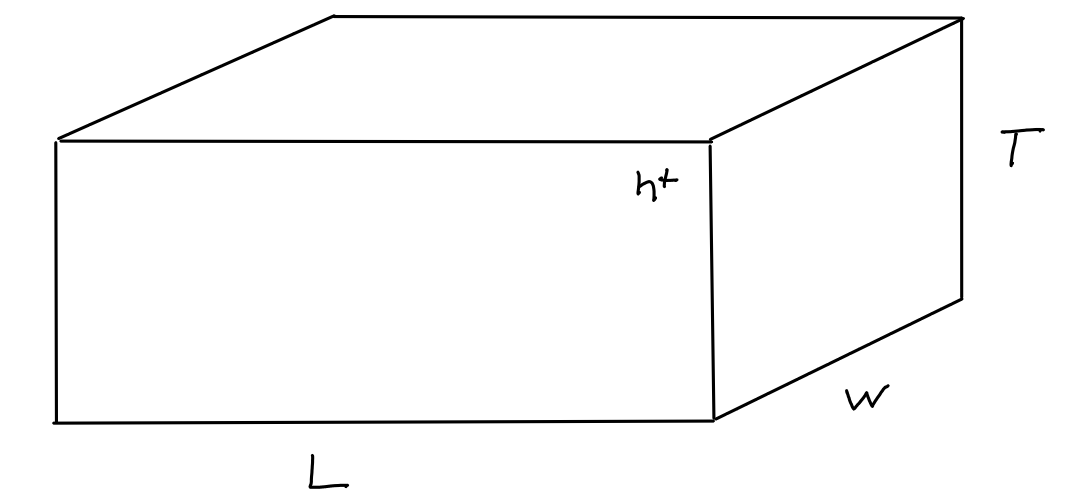
\includegraphics[width=0.4\textwidth]{shrho.png}
\end{wrapfigure}

When we calculate the resistivity of a block of doped silicon like in figure we define $\rho_{sh}=\rho/T$ as the sheet resistivity
\begin{equation}
R=\rho\frac{L}{WT}=\rho_{sh}\frac{W}{L} 
\end{equation}
Diffusion current is driven by a gradient of concentration so the density of current is 
\begin{equation}
J_n=qD_n\frac{dn}{dx} \ \ \ \ J_p=qD_p\frac{dp}{dx}
\end{equation}
where $D_n\ ,D_p$ are the diffusion coefficients defined by Einstein's relations as 
\begin{equation}
D_n=\mu_n\frac{kT}{q}\ \ \ D_p=\mu_p\frac{kT}{q}
\end{equation}
\newline
%------------------------------------------------------------------------%
\section{Bands "geography"}

\centering
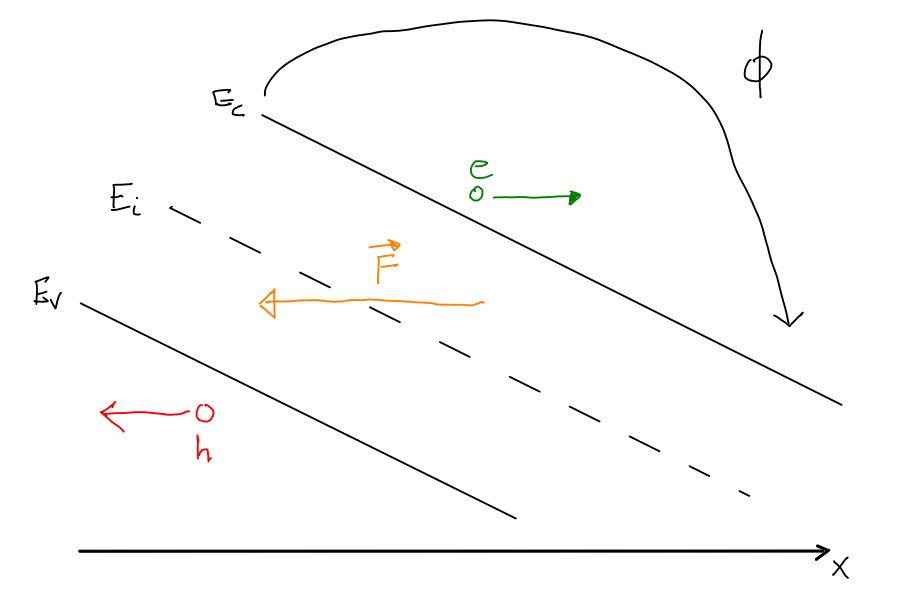
\includegraphics[width=0.5\textwidth]{bandsgeo.png}\\
\raggedright

We can obtain external potential $\phi$ as $\phi=\frac{-E_i(x)}{q}$.\\
The external potential increases in the direction the bands band downwards. The electric field is in the opposite direction of the growth of potential $\vec{F}=-\frac{d\phi}{dx}$.\\
Electrons move by drift in the opposite direction of F and holes in the same direction of F.\\

\centering
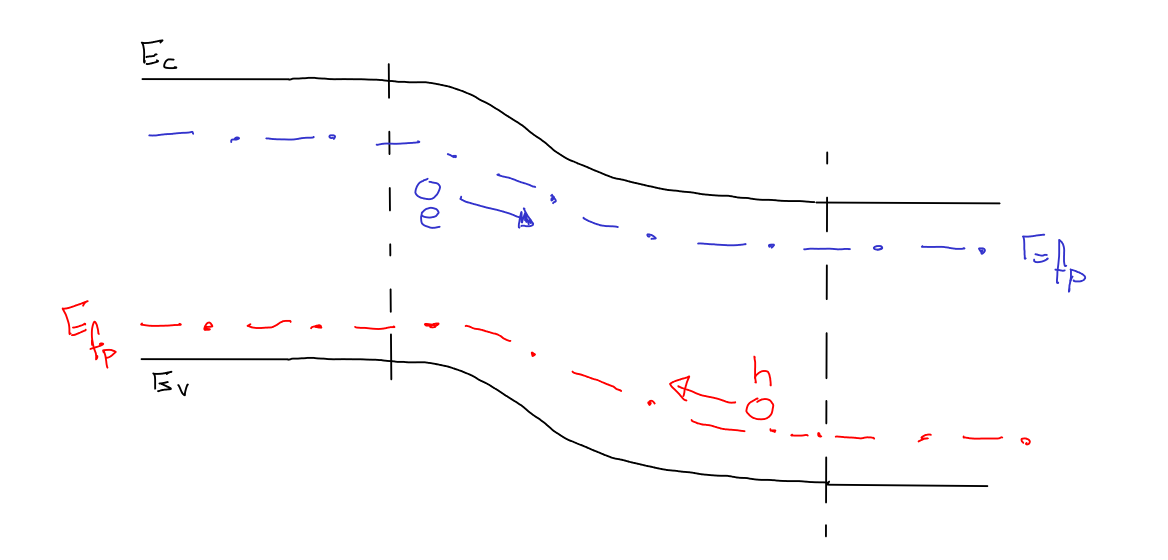
\includegraphics[width=0.5\textwidth]{bandsgeo2.png}\\
\raggedright

Without condition of thermal equilibrium electrons move from regions of high quasi fermi level to regions of low quasi fermi level and holes vice-versa.
%------------------------------------------------------------------------%
\section{Poisson equation}
Poisson equation is important to study the electrostatic of a system.\\
We can derive it from Maxwell's first law 
\begin{equation}
F=-\overrightarrow{\nabla}\phi\rightarrow F=-\frac{d\phi}{dx}
\end{equation}
and Gauss equation
\begin{equation}
\overrightarrow{\nabla}\overrightarrow{F}=\rho/\varepsilon_{Si}
\end{equation}
from witch we obtain considering that all charges we have in a semiconductor are holes, electrons and ionized donors 
\begin{equation}
\frac{d^2\phi}{dx^2}=-\rho/\varepsilon_{Si}=-\frac{q}{\varepsilon_{Si}}(p-n+N_d^+-N_a^-)
\end{equation}
In order to study the electrostatic of a system we have olso to know the coninutity equations of the electric field that are
\begin{equation}
F_{t1}=F_{t2} \Longleftrightarrow \epsilon_1F_{n1}-\epsilon_2F_{n2}=Q'_{int}
\end{equation}
\newline
{\bf Debye length}\\
Band banding is the phenomena caused by applying an electric field on a material at termodinamic equilibrium. This band banding causes different concentrations of e an h over the space so we can re-write the electron and holes concentrations taking in account the change of $\phi(x)$ over the space as
\begin{equation}
n=n_ie^{q\frac{\phi(x)-\phi_f}{kT}} \ \ \ p=n_ie^{q\frac{\phi_f-\phi(x)}{kT}}
\end{equation}
This band banding is tipically caused by the change of doping concentration over the space.With a smooth change of $N_d$ in a material we can assume that $n=N_d$.\\
Let's assume a step-like function in doping concentration in this case we cannot consider $n=N_d$ over the space beacuse this assumption will lead us to an infinite electric field.\\ 
Using Poisson equation and neglecting holes and ionized acceptors we can say that $N_d(x)=\hat{N_d}+\delta N_d(x)$ corrisponding to $\phi(x)=\hat{\phi}+\delta \phi(x)$ and assuming $\delta N_d<<N_d $ we can write
\begin{equation}
\frac{d^2\phi}{dx^2}=-\rho/\varepsilon_{Si}=-\frac{q}{\varepsilon_{Si}}(\hat{N_d}+\delta N_d(x)-n_ie^{q\frac{\hat{\phi}+\delta\phi(x)-\phi_f}{kT}})=-\frac{q}{\varepsilon_{Si}}(\hat{N_d}+\delta N_d(x)-\hat{N_d}-n_ie^{q\frac{\delta\phi(x)}{kT}})
\end{equation}  
we can write the first order expansion of the exponential term beacuse the exponent is small obtaining the following differential equation
\begin{equation}
\frac{d^2\phi}{dx^2}=\frac{q^2\hat{N_d}}{\varepsilon_{Si}kT}\phi(x)-\frac{q}{\varepsilon_{Si}}\delta N_d(x)
\end{equation}
the solution of this equation give us an exponential decrease of the potential with a length called Debye length
\begin{equation}
L_D=\sqrt{\frac{\varepsilon_{Si}kT}{q^2N_d}}
\end{equation}
this will cause a net charge (both negative and positive near the discontinuity.\\
%------------------------------------------------------------------------%
\section{Quasi-Fermi levels}

\begin{wrapfigure}{i}{0pt}
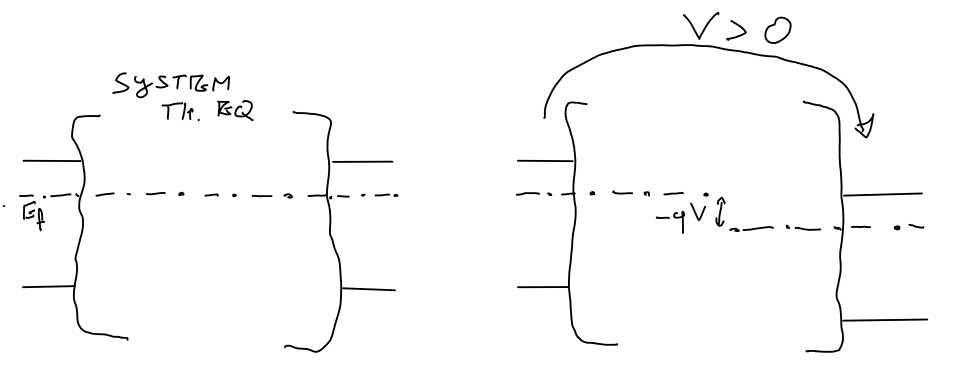
\includegraphics[width=0.4\textwidth]{perturbation.png}
\end{wrapfigure}

For having a net current transport (we're leaving the thermodinamic equilibrium hypotesis) we have to perturbe our system by for example applying at the contact (:region of dispositive from witch we can externally apply a F, a good contact stay at th. eq.) a $V\neq 0$. 
As the figure shows  we can't introduce a $E_f$ level and so we cannot use the FD distribution. If the perturbation is weak we can recover all expressions of th.eq by introducing different Fermi levels both for e and h called quasi Fermi levels
\begin{equation}
n=n_ie^{\frac{E_{fn}-E_i}{kT}} \ \ \ \ \ \ p=n_ie^{\frac{E_i-E_f}{kT}}
\end{equation}
so we can write the law of mass action generalized as 
\begin{equation}
pn=n_i^2e^{\frac{E_{fn}-E_{fp}}{kT}}
\end{equation}
Now let's try to analise the total current density of electrons. The formula has a strong dependance from the electrostatic potential (from F and n) so
\begin{equation}
J_n=-qn\mu_nF+qD_n\frac{dn}{dx}=-qn\mu_n\frac{d\phi}{dx}+qD_n\frac{d}{dx}\left(n_ie^{q\frac{\phi-\phi_f}{kT}}\right)=-qn\mu_n\frac{d\phi_f}{dx}
\end{equation} 
But since the Fermi potential is costant the result is 0 and it's obvius beacuse we assume th.eq. with formula (1.20).
If we substitute the (1.39) in n we obtain
\begin{equation}
J_n=-qn\mu_n\frac{d\phi_{fn}}{dx}
\end{equation}
that isn't 0 beacuse $\phi_{fn}$ can change.\\
Electrons moves from the region of high quasi Fermi level to region of low quasi Fermi level, holes the opposite.
\newline
%------------------------------------------------------------------------%
\section{Equation of for e and h}

\centering
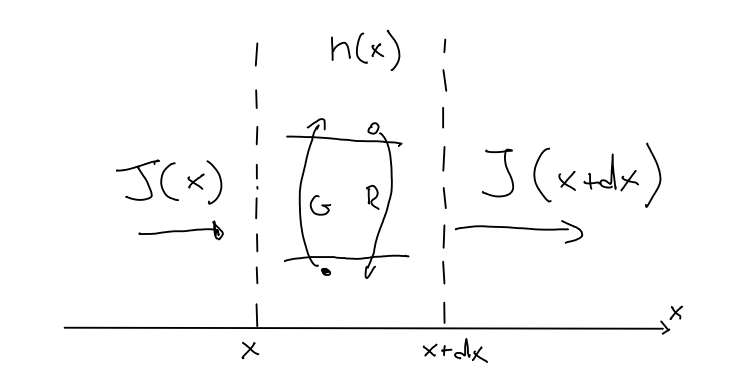
\includegraphics[width=0.4\textwidth]{continuityeq.png}\\
\raggedright

Let's consider the figure above if we make a ballace of charges between x and x+dx we have 
\begin{equation}
\frac{\partial n}{\partial t}dx=-J_n(x)/q+J_n(x+dx)/q-(G-R)dx
\end{equation}
where G and R are generation and ricombination processes per unit time per unit volume. If we expand at the first order $J(x+dx)$ and simplify the expression we have
\begin{equation}
\frac{\partial n}{\partial t}=\frac{1}{q}\frac{\partial J_n}{\partial x}+G-R \ \ \ \ \ \ \frac{\partial p}{\partial t}=-\frac{1}{q}\frac{\partial J_p}{\partial x}+G-R
\end{equation}
that are the continuity equation for electrons and hole current.\\
In a stationary system nothing change with time so subtractring the 2 equation we have 
\begin{equation}
\frac{1}{q}\frac{\partial(J_n+J_p)}{\partial x}=0
\end{equation}
so the sum of the 2 contributions of current from e and h stay costant. If we neglect G and R the 2 contrbutes are costant separatly.\\
G and R process restabilize equilibrium of a system if we perturb the minority carrier concentration. If we disturb majority carrier the system returns in equilibrium with a very short time costant.
Let's analyse the 2 case.\\ 

%------------------------------------------------------------------------%
{\bf Majority carrier perturbation}\\
Assume a n-doped material and let us add $\Delta n$ concentration of electrons. Using poisson equation we have
\begin{equation}
\frac{\partial \phi^2}{\partial x^2}=-\frac{q}{2\varepsilon}\left(-n-\delta n + N_d\right)=\frac{q\Delta n}{\varepsilon}=-\frac{dF}{dx} 
\end{equation}
from this result we obtain a field that has a linear dependence over the space that tends to move away the excess of charge with a drift current (no diffusion the concentration is costant) so using  1.44
\begin{equation}
\frac{\partial J_n}{\partial x}=qn\mu_n\frac{\partial F}{\partial x}
\end{equation}
\begin{equation}
\frac{\partial n}{\partial t}=\frac{1}{q}\frac{\partial J_n}{\partial x}=\frac{-1}{q}qn\mu_n\frac{q\Delta n}{\partial \varepsilon}=-\frac{\Delta n}{\varepsilon \rho}
\end{equation}
solving this differential equation we have a solution that has an exponential dependence with $\varepsilon \rho$ that is called the dialectric relaxation time of the material; it's the time costant that the system use to return to its equilibrium ($\simeq ps$)\\

%------------------------------------------------------------------------%
{\bf Minority carrier perturbation}\\
The phenomena described for majority carrier concentration isn't valid for minority carrier. Considering a n-doped material like before the $\rho$ in equation 1.48 is very high (we are considering holes now) so the real result of the field is that attracts a concentration $\Delta n$ over $\Delta p$ creating a quasi-neutral region where G and R slowly decrease the 2 extra concentration.\\
In the processes of G and R in Si electrons cannot move thought the bandgap from CB to VB they need another particle to respect the conservation of momentum.\\

\begin{wrapfigure}{i}{0pt}
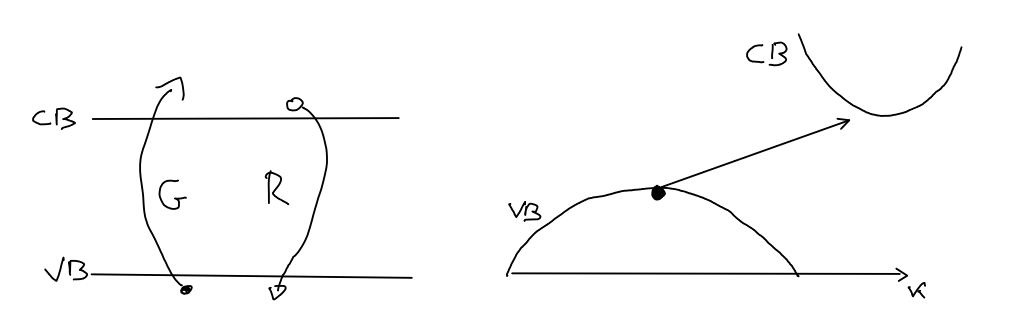
\includegraphics[width=0.4\textwidth]{srhp1.png}
\end{wrapfigure}

We need a difect of the cristal that creates another "band" in the bandgap this process called difect assisted and is described by Shockley-Reed-Hall theory.\\
The difect can only be empty or filled with one electron so there can be only 4 process: 1)Difect empty captures e from CB   2) Difect filled realeses an e to CB 3) Difect filled captures hole from VB 4) Difect empty realeses an hole from VB.

\begin{wrapfigure}{i}{0pt}
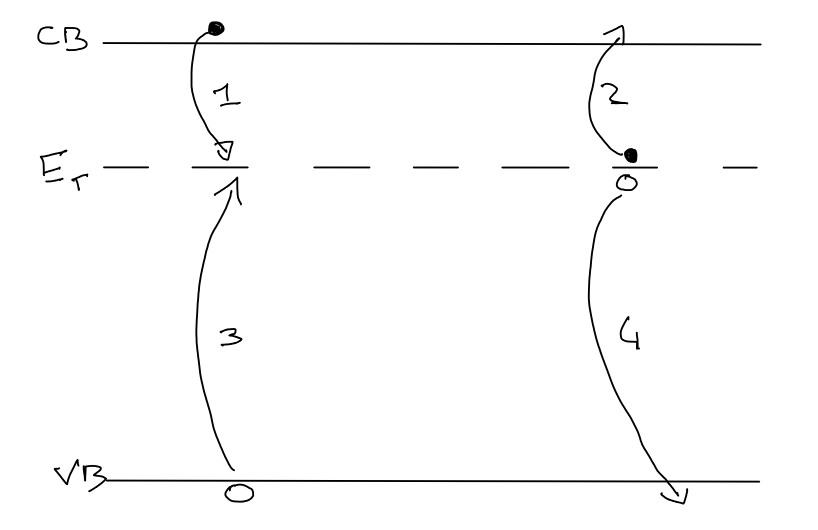
\includegraphics[width=0.4\textwidth]{srhp2.png}
\end{wrapfigure}

For R we need 1+3 for G 2+4.\\
The rate of 1 can be described as 
\begin{equation}
r_1=N_T(1-f(E_T))n(v_{th} \delta_n)
\end{equation}
where: $N_T$ is the total difect concentration ,f probability of the difect to be filled and the last term is a costant where $\delta_n$ is the capture crossection.\\
The rate of process 2 can be described as 
\begin{equation}
r_2=N_Tf(E_T)e_n
\end{equation}
where $e_n$ is a proportionality costant emission rate for e.
Under th.eq. $r_1=r_2$ and we can use the FD distribution for f. Under this condition we can calculate $e_n$ (and using the same consideration olso $e_p$)
\begin{equation}
e_n=n_iv_{th}\delta_ne^{\frac{E_T-E_i}{kT}} \ \ \ \ \ \ e_p=n_iv_{th}\delta_pe^{\frac{E_i-E_T}{kT}}
\end{equation}
So assuming $\delta_p=\delta_n=\delta$ and $\tau=1/(v_{th}N_T\delta)$ under stationary condition $R=r_1-r_2=r_3-r_4$ from this we obtain $f(E_T)$ and 
\begin{equation}
R=\frac{pn-n_i}{\tau\left[p+n+2n_iCosh(\frac{E_T-E_i}{kT})\right]}
\end{equation}
re-writing the numerator we can obtain that if $E_{fn}>E{fp}\rightarrow R>0$ and if $E_{fn}<E{fp}\rightarrow R<0$.\\
Looking at the graph of G and R 

\centering
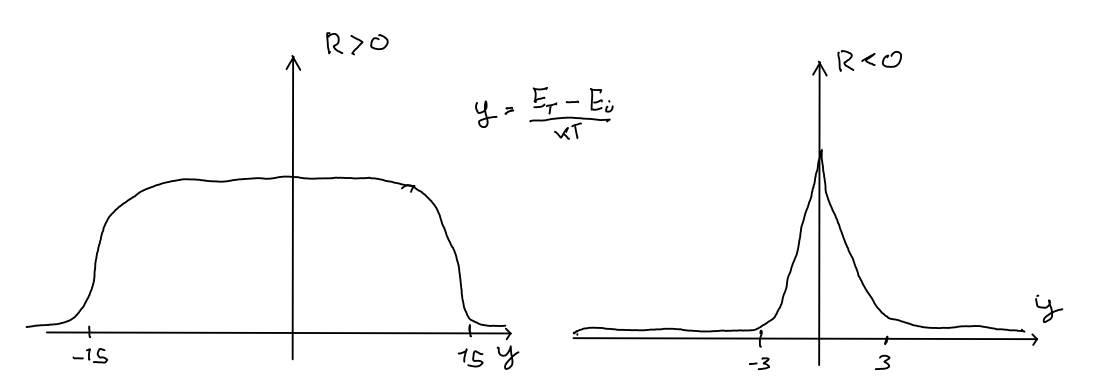
\includegraphics[width=0.4\textwidth]{RG.png}\\
\raggedright

[...]

\section{Quasi-neutral condition}
Under quasi-neutral condition $\Delta n +n_0=n$ and $\Delta p +p_0=p$ assuming low injection level ($\Delta n<<p_0+n_0$) we can neglect in the eq of R all the terms with "$\Delta$" so we obtain
\begin{equation}
R=\frac{\Delta n}{\tau_n}=\frac{(p_0+n_0)\Delta n}{\tau\left[p_0+n_0+2n_iCosh(\frac{E_T-E_i}{kT})\right]}
\end{equation}
if we suppose $E_T-E_i0=0$\\
So the continuity equation for electrons becomes
\begin{equation}
-\frac{d\Delta n}{dt}=R \rightarrow \Delta n \propto e^{-t/\tau_n}
\end{equation} 
where $\tau_n$ is dipendent on the quality of the material

